% !TEX encoding = UTF-8 Unicode
\documentclass[a4paper]{article}

\usepackage{color}
\usepackage{url}
\usepackage[T2A]{fontenc} % enable Cyrillic fonts
\usepackage[utf8]{inputenc} % make weird characters work
\usepackage{graphicx}
\usepackage{multirow}
\usepackage[english,serbian]{babel}
%\usepackage[english,serbianc]{babel} %ukljuciti babel sa ovim opcijama, umesto gornjim, ukoliko se koristi cirilica

\usepackage[unicode]{hyperref}
\hypersetup{colorlinks,citecolor=green,filecolor=green,linkcolor=blue,urlcolor=blue}

\usepackage{listings}
\usepackage{multirow}
\newcommand\todos[1]{\textcolor{red}{#1}}

%\newtheorem{primer}{Пример}[section] %ćirilični primer
\newtheorem{primer}{Primer}[section]

\definecolor{mygreen}{rgb}{0,0.6,0}
\definecolor{mygray}{rgb}{0.5,0.5,0.5}
\definecolor{mymauve}{rgb}{0.58,0,0.82}

\lstset{ 
  backgroundcolor=\color{white},   % choose the background color; you must add \usepackage{color} or \usepackage{xcolor}; should come as last argument
  basicstyle=\footnotesize,        % the size of the fonts that are used for the code
  breakatwhitespace=false,         % sets if automatic breaks should only happen at whitespace
  breaklines=true,                 % sets automatic line breaking
  captionpos=b,                    % sets the caption-position to bottom
  commentstyle=\color{mygreen},    % comment style
  deletekeywords={...},            % if you want to delete keywords from the given language
  escapeinside={\%*}{*)},          % if you want to add LaTeX within your code
  extendedchars=true,              % lets you use non-ASCII characters; for 8-bits encodings only, does not work with UTF-8
  firstnumber=1000,                % start line enumeration with line 1000
  frame=single,	                   % adds a frame around the code
  keepspaces=true,                 % keeps spaces in text, useful for keeping indentation of code (possibly needs columns=flexible)
  keywordstyle=\color{blue},       % keyword style
  language=Python,                 % the language of the code
  morekeywords={*,...},            % if you want to add more keywords to the set
  numbers=left,                    % where to put the line-numbers; possible values are (none, left, right)
  numbersep=5pt,                   % how far the line-numbers are from the code
  numberstyle=\tiny\color{mygray}, % the style that is used for the line-numbers
  rulecolor=\color{black},         % if not set, the frame-color may be changed on line-breaks within not-black text (e.g. comments (green here))
  showspaces=false,                % show spaces everywhere adding particular underscores; it overrides 'showstringspaces'
  showstringspaces=false,          % underline spaces within strings only
  showtabs=false,                  % show tabs within strings adding particular underscores
  stepnumber=2,                    % the step between two line-numbers. If it's 1, each line will be numbered
  stringstyle=\color{mymauve},     % string literal style
  tabsize=2,	                   % sets default tabsize to 2 spaces
  title=\lstname                   % show the filename of files included with \lstinputlisting; also try caption instead of title
}

\begin{document}

\title{Privatnost i njena zaštita u digitalnom dobu\\ \small{Seminarski rad u okviru kursa\\Metodologija stručnog i naučnog rada\\ Matematički fakultet}}
\author{Đaković Branko, Krčmarević Mladen,\\Petrović Ana, Spasojević Đorđe\\brankodjakovic08@gmail.com, mladenk@twodesperados.com,\\ pana.petrovic@gmail.com, djordje.spasojevic1996@gmail.com}

%\date{9.~april 2015.}

\maketitle

\abstract{ Pojavom interneta definicija privatnosti postaje sve šira i sve labavija. Uzimajući u obzir da velika većina ljudi koristi internet svakodnevno, problem privatnosti na internetu i količine informacija koja se na njemu svakodnevno deli jedan je od većih problema današnjice, zbog čega je vredan dubljeg razmatranja. Cilj ovog rada je bio upravo skretanje pažnje na ovaj problem, kao i razmatranje podataka i nalaza istraživanja koja se bave privatnošću i percepcijom korisnika o njoj. Ključne reči: privatnost, internet privatnost, zaštita privatnosti, društvene mreže, privatnost podataka.  
} 
\tableofcontents

\newpage

\section{Uvod}
\label{sec:uvod}  
\par U martu 2018. godine bivši zaposleni firme Kembridž Analitika (eng.\\~{\em Cambridge Analytica}) je otkrio javnosti da je ova firma kupila od društvene mreže Fejsbuk privatne podatke barem 50 miliona korisnika bez njihove saglasnosti \cite{guardian}. Podaci su prikupljeni uz pomoć aplikacije na Fejsbuku koja je bila namenjena prikupljanju podataka u akadamske svrhe. Međutim, ova aplikacija je, osim za one korisnike koji su na to pristali, uzimala podatke i svih njihovih prijatelja. Postoje sumnje koje nisu potvrđene da su ovi podaci zloupotrebljavani na različite načine, kao što je na primer njihovo korišćenje tokom predsedničke kampanje Donalda Trampa, kao i tokom perioda referenduma o članstvu Ujedinjenog Kraljevstva u Evropskoj uniji. Politika platforme Fejsbuk izričito zabranjuje prodaju ili korišćenje podataka korisnika u svrhe oglašavanja, što je učinilo ovaj slučaj jednim od najvećih slučaja kršenja privatnosti podataka na internetu. Iako optužbe da su podaci korišćeni u predsedničkoj kampanji nisu potvrđene i načelno ne moraju biti tačne, ova vest je otvorila diskusije o tome ko i u kolikoj meri ima pristup našim podacima na internetu.
\par Uzimajući u obzir da društvene mreže imaju milijardu korisnika na mesečnom nivou, količina privatnih podataka koje oni ostavljaju na ove platforme, a koji se kreću od uzrasta i lokacije, do interesovanja i hobija, je ogromna \cite{instagram}. Uz to, ove kompanije najčešće ne traže dozvolu da čuvaju podatke korisnika, ili kada je traže, to rade na netransparentan način. Povrh svega toga, pojedinci najčešće nisu ni svesni da sve što ostave na internetu, kasnije može biti iskorišćeno na načine koji bi u nekim slučajevima mogli da idu i na njihovu štetu.
\par Iako problem privatnosti nije nov, razvoj tehnologije i interneta je mnoge aspekte ovog problema proširio i doveo na sasvim novi nivo, zbog čega je ova tema često predmet debate. Cilj ovog rada je da da pregled raznih aspekata problema privatnosti na internetu, kao i da pokuša da detaljnije objasni i približi čitaocu razloge zbog kojih bi trebalo da se interesuje za privatnost svojih podataka na internetu. U tu svrhu, u radu se najpre razmatra konceptualna definicija privatnosti, a zatim se problem privatnosti posmatra iz zakonskog ugla. Nakon toga, biće predstavljeni najčešći oblici narušavanja privatnosti na internetu, kao i rizici po privatnost korisnika. Na kraju, biće date i mogućnosti zaštite privatnosti na internetu koje su na raspolaganju. U zaključku je razmotren problem u celini, a dati su i predlozi toga na koji način bi privatnost na internetu trebalo razmatrati u budućnosti.

\section{Šta je privatnost?}
\label{sec:prvoPoglavlje}
Pravo na privatnost se smatra jednim od najjasnijih i najvrednovanijih ljudskih prava, ali je privatnost koncept koji je teško definisati \cite{solove}. Jedan od problema u definisanju privatnosti leži u širini i neodređenosti ovog pojma, koji obuhvata zaštitu od ispitivanja i nedozvoljenih pretraga, kontrolu nad sopstvenim telom i privatnim informacijama, pa čak i pravo na slobodu mišljenja i govora. Ključni pojam u raspravama o tome šta je privatnost je koncept pristupa, bilo u kontekstu fizičke bliskosti nekoj osobi, bilo u kontekstu posedovanja znanja o toj osobi \cite{ethics}. Pristup podrazumeva da jedna osoba ima pravo da ograniči ili zabrani pristup sebi u najširem smislu te reči, dok sa druge strane, on takođe podrazumeva i pravo drugih da ostvare pristup određenoj osobi. Upravo je sukob između ova dva ono u čemu leži suština privatnosti. Taj sukob se najviše reflektuje u suprotstavljanju  privatnog i javnog, i onoga što bi trebalo da bude privatno i javno. Sa jedne strane, svaki pojedinac ima pravo da ograniči informacije o sebi koje su deo javnog znanja, međutim, preveliko ograničenje pristupa može dovesti do zloupotrebe i do loših posledica po društvo. Upravo zato privatnost predstavlja ključan problem slobode i demokratije \cite{solove}. Zbog toga ni ne čudi što se ogroman broj zakona i ustavnih prava odnosi upravo na privatnost. Uz to se sprovođenje ovih zakona i odredbi dovodi u pitanje usled nedefinisanosti pojma. Iako je usled pomenutih problema teško dati preciznu definiciju, jedan od mogućih načina da definišemo privatnost je da je konceptualizujemo kao društveni ugovor koji dozvoljava pojedincu da ima određen nivo kontrole nad time ko i u kojoj meri ima pristup ne samo njegovim podacima, već i njegovom telu \cite{ethics}.

\subsection{Privatnost na internetu}
\label{subsec:privatnostNaInternetu}
Kao što je već pomenuto, sa razvojem interneta, problem shvatanja privatnosti se dodatno komplikuje  i činjenica  da  veliku  većinu  dana  provodimo  na  internetu  donosi nove  aspekte  problemu  privatnosti. Svakog  dana, korišćenjem interneta za različite potrebe, svaka osoba ostavlja za sobom elektronski trag svojih aktivnosti, koje mogu biti takve da otkrivaju i identitet pojedinca. Uz to, ostavljanje privatnih podataka može imati i određene prednosti, kao što su personalizovane poruke ili na primer, popusti, te je pojedinac suočen sa odlukom da li da propusti ove prednosti, ali očuva privatnost ili da ostavi svoje podatke na internetu, koji kasnije mogu biti zloupotrebljeni kako bi ostvario pogodnosti koje mu se nude \cite{renata}.
\par Povrh ovih informacija koje sami voljno ili nevoljno ostavljamo na internetu, danas su i informacije koje su deo javnih informacija (kao što su podaci o rođenju ili bračnom statusu pojedinca) kompjuterizovane, što ih čini daleko dostupnijim. Sa jedne strane, ovo ima svoju jasnu prednost, ali ovo podrazumeva i to da su ove informacije daleko pristupačnije i onima kojima možda ne bismo želeli da budu \cite{ethics}. Kapacitet prikupljanja podataka svakim danom sve više raste, što dovodi  do mnogo lakšeg prepoznavanja pojedinca i korišćenja podataka o njemu u različite svrhe. Iako često sami odlučujemo da podelimo neke privatne informacije na internetu, korisnik nije ni svestan kada daje dozvolu nekoj privatnoj kompaniji da koristi njegove informacije i najčešće su pojedinci zbunjeni oko toga šta su tačno njihova prava na privatnost na internetu \cite{renata}.

\subsection{Percepcija privatnosti}
\label{subsec:percepcija}
Bitan aspekt razmatranja privatnosti na internetu je koncept percipirane privatnosti. Odnosno, problem privatnosti ne ostaje samo na tome da li ona postoji ili ne,  već se širi i na to da li pojedinac vidi svoju privatnost kao problem i ako da, u kojoj meri. Percepcija privatnosti dalje određuje ponašanje pojedinca na internetu,  utoliko što će pojedinci biti spremniji da koriste određene veb stranice ukoliko smatraju da je njihova privatnost zaštićena i obrnuto. Povrh toga, pokazuje se da, kada postoji uverenost da je privatnost pojedinca zaštićena, oni su spremni da je se vrlo lako odreknu, radi ispunjenja nekih potreba (kao što je na primer kupovina).
\par Percepciju privatnosti na internetu oblikuju različiti faktori, od kojih se neki vezuju za samog pojedinca, neki za same stranice koje korisnici posećuju, a neki  za datu situaciju. Tako, shvatanje privatnosti može zavisiti od pola ili uzrasta, ali i obrazovanja pojedinca, prethodnog iskustva na internetu kao i od toga da li je osoba prethodno iskusila narušavanje privatnosti na internetu. Isto tako, to da li će pojedinac biti zabrinut za svoju privatnost na određenom sajtu može zavisiti od poznatosti brenda tog sajta, opaženog integriteta ili opaženog rizika tog sajta. Na kraju, to kako percipiramo trenutnu pretnju po privatnost može da zavisi i od toga kakvo je poklapanje izmedu traženih informacija i usluge koju dobijamo i da li nam je ona smislena, ili od trenutne percepcije toga koliko je određeni podatak koji ostavljamo na internetu osetljive prirode \cite{renata}. Dakle, percepcija privatnosti na internetu je širok problem, koji je pod uticajem mnogih faktora, a koji povratno utiče na ponašanje svakog pojedinca na internetu, koje ponovo dovodi do narušavanja ili očuvanja privatnosti na internetu, te je stoga ovaj problem veoma relevantan za razumevanje privatnosti na internetu danas.  

\section{Privatnost i društvene mreže}
\label{sec:drugoPoglavlje}
Kao što je u prethodnom poglavlju prikazano, privatnost predstavlja problem kako pojedinca, tako i društva. Zbog toga treba razmotriti najčešće probleme sa kojima se čovek suočava kada koristi internet, što je za većinu svakodnevno, odnosno treba razmotriti u kojim to aspektima je za prosečnog korisnika privatnost najčešće ugrožena.
\par Oko dve trećine korisnika interneta koristi društvene mreže, te je samim tim problem privatnosti upravo na društvenim mrežama sve aktuelniji \cite{sm1}. Mnoge društvene mreže nude različita podešavanja privatnosti, te se čini da je odluka o tome da li i u kojoj meri želi da podeli informacije o sebi ipak na korisniku. I zaista, istraživanja pokazuju da ljudi sve češće i više preduzimaju korake da ograniče pristup svojim privatnim informacijama. Tako je pokazano da je broj korisnika koji su obrisali komentare drugih ili skinuli svoje ime sa slika na kojima su označeni u porastu u odnosu na 2006. godinu. Više od polovine korisnika ima privatne profile, što ograničava broj ljudi koji mogu da vide njihov sadržaj samo na one koje oni odaberu. Pri tome, žene češće imaju privatne profile, što znači da su one više zabrinute za svoju privatnost u odnosu na muškarce.
\par Uzimajući u obzir da su najaktivniji korisnici društvenih mreža mladi ljudi, ne čudi što se veliki broj istraživanja fokusira upravo na mlade. Podaci pokazuju da su tinejdžeri 2012. godine bili daleko spremniji da podele informacije o sebi nego što su to bili tinejdžeri 2006. godine \cite{sm2}. U tabeli \ref{tab:tabela1} dat je prikaz odnosa te dve godine i količine informacija koje su oni javno objavili. Uz to, mladi su samouvereni u svoju sposobnost da kontrolišu broj informacija koje drugi mogu da vide o njima.
\par Međutim, postavlja se pitanje da li zaista korisnik ima toliku kontrolu nad informacijama koje drugi vide o njemu, uprkos samouverenosti da to kontroliše. Istraživanja pokazuju da bez obzira na to koliko neko odluči da deli informacija, to šta njegovi prijatelji odluče da dele takođe igra značajnu ulogu, čak iako pojedinac nema nalog na društvenim mrežama. Prema tome, sa pojavom društvenih mreža problem privatnosti je postao daleko difuzniji i nejasniji nego što je bio do tada i moguće je postaviti pitanje da li izostanak sa društvenih mreža uopšte garantuje privatnost i da li ona danas uopšte postoji.
\\



\begin{table}[h!]
	\begin{center}
		\caption{Procenti tinejdžera koji su delili svoje podatke na društvenim mrežama 2006. i 2012. godine}
		\begin{tabular}{|c | c c c c c|} \hline
			
Godina & \begin{tabular}[x]{@{}c@{}} Sopstvena \\fotografija \end{tabular} & \begin{tabular}[x]{@{}c@{}} Naziv \\ škole \end{tabular} & \begin{tabular}[x]{@{}c@{}}Mesto \\ stanovanja \end{tabular} & \begin{tabular}[x]{@{}c@{}}Imejl \\ adresa \end{tabular} & \begin{tabular}[x]{@{}c@{}}Broj \\ telefona \end{tabular} \\
			\hline
			2006 & 79\% & 49\% & 61\% & 29\% & 2\% \\
			2012 & 91\% & 71\% & 71\% & 53\% & 20\%\\
			\hline
		\end{tabular}
		\label{tab:tabela1}
	\end{center}
\end{table}

\subsection{Krađa identiteta}
Uzimajući u obzir prethodno pomenutu količinu informacija koju su ljudi spremni da podele na internetu, kao i činjenicu da ona raste, dolazi do porasta fenomena krađe identiteta. Krađa identiteta je u porastu poslednjih godina, s obzirom da svaki profil na društvenoj mreži pruža dovoljan broj informacija za prisvajanje nečijeg identiteta, makar površno. Spam mejlovi su jedan od popularnijih načina na koji se uzimaju informacije o nekoj osobi, pa je tako slanje masovnih mejlova sa lažnim linkovima ka određenim sajtovima veoma često, toliko da postoji oko 30 ovakvih napada dnevno, koji potencijalno mogu da oštete hiljade ljudi \cite{it1}. Međutim, postoje i procesi koji su velikom većinom automatski, te samim tim veoma efikasni u dostizanju velikog broja ljudi, što može imati dalekosežne posledice \cite{it2}. Ovo omogućava uverljivu simulaciju identiteta neke osobe, a lakoća sa kojom je moguće ovo izvršiti je zabrinjavajuća.
\par Kako napreduje tehnologija, tako se načini na koje je moguće ukrasti nečiji identitet usložnjavaju i pružaju više opcija za zloupotrebu. Jedna od takvih opcija je dipfejk (eng.~{\em deepfake}) sadržaj i tehnologija. Korišćenje algoritama za mašinsko učenje i open source koda, postoji mogućnost da se manipuliše video sadržajem, tako da je moguće njegovo menjanje da sadrži lice bilo koje osobe \cite{it3}.  S obzirom da većina korisnika ima veliku količinu svojih slika na internetu, ne čudi što je javni diskurs bogat raspravama o dipfejku, do te mere da postoji predlog zakona u Americi da se ova tehnologija zabrani. Dipfejk video zapisi otvaraju sasvim novo polje za krađu identiteta, koje nije tako lako prepoznati i čije je posledice teško ispraviti. Ovi video sadržaji bi tako mogli da prikazuju političke lidere ili druge značajne ličnosti kako govore ili rade bilo šta, što može imati izuzetno nepovoljne posledice po širu javnost. Iako se čini da je maliciozni potencijal ove tehnologije veliki, ipak ne postoji mnogo potencijalno opasnih sadržaja ove vrste \cite{it4}. Ipak, oni se sve češće koriste u svrhe sajber nasilja, što znači da ih ne treba ignorisati i da treba imati na umu da privatnost na internetu može biti narušena i na ovaj način, kao i da broj mogućnosti zloupotrebe privatnih informacija korisnika u različite svrhe svakodnevno raste.  

\subsection{Kolačići}

Prilikom upotrebe pregledači veba na računar korisnika smeštaju kolačiće (eng.~{\em cookies}) \cite{cookies1}. Kolačići su male tekstualne datoteke koje čuvaju informacije o veb sajtovima kao što su na primer informacije o prijavi korisnika, sadržaj korpe prilikom  kupovine, jezik i ostale informacije koje čine korišćenje interneta jednostavnijim. U zavisnosti od trajanja postoje sesijski, odnosno kratkotrajni kolačići koji bivaju izbrisani prilikom gašenja prgledača i trajni kolačići koji imaju rok trajanja, te se čuvaju na računaru do isteka tog roka. U okviru trajnih, kolačići se dele na kolačiće prve strane i kolačiće treće strane.  Kolačići prve strane se koriste samo od strane veb sajtova koji su ih napravili i prvenstveno se koriste za poboljšanje korisničkog iskustva. Kolačići treće strane (nazivaju se i kolačići za praćenje) koriste  sajtovi koji ih nisu napravili. To omogućava subjektima koji su napravili kolačić da dobiju informacije svaki put kada korisnik poseti neku stranicu na kojoj oni poseduju resurse. Obično je korisno da veb sajtovi pored sadržaja koji je napravio vlasnik koriste resurse drugih sajtova kako bi dodali određene  funkcionalnosti. Najčešće su baš ti resursi oni koji vrše praćenje na internetu. Uz to, kako kolačići omogućavaju i drugim sajtovima pristup informacijama, tako korisnici mogu videti oglase koji su povezani sa njihovim prethodnim kupovinama, iako nisu pristali direktno da te informacije podele sa tim konkretnim sajtom. Sama praksa kolačića je do skoro bila implicitna, odnosno zahtevala je od korisnika da sam isključi opciju kolačića, umesto da privatnost bude pretpostavka od koje se polazi. Od skoro je ovaj problem i zakonski regulisan, te sada svi sajtovi moraju da obaveste korisnika da prikupljaju informacije o njima putem kolačića i moraju da dobiju pristanak samog korisnika da to urade. Međutim, uprkos ovoj praksi, kao i postojanju prakse stavljanja natpisa da je privatnost podataka zagarantovana, većina ispitanika to ne prepoznaje kao pozitivno i kao nešto što uliva sigurnost \cite{cookies2}. Naprotiv, korisnici izveštavaju da im nisu jasne politike privatnosti, koje retko čitaju, kao ni načini na koje je njihova privatnost zagrantovana.
\par Najzastupljeniji resursi koji koriste kolačiće za praćenje su reklame, vidžeti (programčići/aplikacije) društvenih mreža kao što su “podeli” I “sviđa mi se” i veb analitike. Ako ne postoje, i kolačići prve i treće strane se prave prilikom učitavanja sajta, a ukoliko postoje šalju vlasniku kolačića. To znači da nije neophodno da se pritisne na reklamu ili dugme društvene mreže da bi vlasnik resursa dobio kolačić za praćenje, a time i informacije o sajtu koji je korisnik posetio, a nekad i sajtu sa koga je došao do trenutnog. Informacije koje kolačići za praćenje mogu da čuvaju obuhvataju istoriju pretraživanja, kupovine, lokacije, informacije o uređajima, kada i gde je viđena prethodna reklama, linkovi na koje je korisnik kliknuo i slično. 
\par Postoji više načina za zaštitu od kolačića. Jedan od načina je korišćenje pregledača u privatnom režimu rada. Međutim, to onemogućava i kolačiće prve strane koji mogu biti korisni. Drugi način koji omogućava da se isključe samo kolačići treće strane je da se obrišu kolačići, a zatim onemogući čuvanje kolačića u podešavanjima pregledača. 


\section{Odnos države prema privatnosti pojedinca}	
\label{sec:trecePoglavlje}
\par Međutim, privatnost na internetu nije samo lični problem pojedinca, već ima daleko šire razmere koji dostižu i nivo same države. Stoga, kada se govori o privatnosti na internetu, treba pomenuti i odnos države i državnih institucija prema privatnosti pojedinca. Kroz istoriju je bio čest slučaj da su države narušavale  privatnost pojedinaca kako bi ostvarile određene interese, rešile određene probleme ili u situacijama ekstremne opasnosti, kao što je na primer borba protiv terorizma. Ovome u prilog ide i činjenica da je slučajeva u kojima su američka administracija i službe kršile privatnost građana bilo mnogo, od prodaje podataka službenika tajnih službi novinarima i privatnim detektivima, do ilegalnog prisluškivanja američkih i stranih državljana od strane FBI-ja.
\par Neki od tih slučajeva su zloupotreba popisnih spiskova od strane američke vojske u Prvom i Drugom svetskom ratu, korišćenje policijskih dronova, kao i televizijske kamere zatvorenog kruga (eng.~{\em closed-circuit television, CCTV}). O ovome svedoči i podatak da prosečan stanovnik Velike Britanije bude uhvaćen na kameri u proseku 300 puta dnevno \cite{ethics, london}. Ne samo da pojedinac može biti uhvaćen na kameri, već se dešava i da država prisluškuje ono što određeni pojedinci u svakom trenutku govore. Iako je prisluškivanje razgovora i postavljanje bubica aktom američkog kongresa iz 1934. godine zabranjeno, osim u slučajevima kada postoji sudski nalog, to nije sprečilo FBI da nastavi da to radi ilegalno, čak i tokom Drugog svetskog rata uz dozvolu predsednika Ruzvelta \cite{ruzvelt}. Nakon rata, nacionalna sigurnosna agencija (eng.~{\em National Security Agency, NSA}), FBI i druge bezbednosne službe nastavile su sa kršenjem zakona o privatnosti pojedinaca, što se kasnije i proširilo na druge vidove komunikacije, i pre svega na internet.

\subsection{Zakoni koji narušavaju privatnost}
\label{subsec:zakoni}
\par Usled pretnje po bezbednost SAD-a, donošeni su zakoni koji su bezbednosnim službama dali veća ovlašćenja, koja su automatski dozvoljavala ovim organizacijama upad u privatnost pojedinaca. Američka administracija je 1978. godine donela zakon o nadzoru stranih službi (eng.~{\em Foreign Intelligence Surveillance Act, FISA}), kojim se dozvoljava tajni nadzor inostranih vlada i njihovih službi. Ovim zakonom američki predsednik je mogao da odobri elektronski nadzor stranih državljana na jednu godinu, pod uslovom da se time ne krši privatnost državljana Amerike. U suprotnom, administracija bi morala da dobije sudski nalog za prisluškivanje. Međutim, bez obzira na postojanje ovog zakona, postoje mnogi slučajevi kršenja njegovih odredbi. Tako je 2013. godine Edvard Snouden, bivši zaposleni u NSA i FBI-ju, obelodanio  na  hiljade  tajnih  dokumenata  američkih tajnih službi, među kojima se našao i projekat PRISM, koji je dozvoljavao NSA pristup mnogim serverima pojedinih internet kompanija, kao i velikoj količini privatnih informacija, među kojima su bili i video pozivi kojima je ovim odredbama dozvoljen pristup čak i bez sudskog naloga \cite{prism}. U odeljku \ref{subsec:prism} detaljno će biti prikazan projekat PRISM.
\par Zakon o skladištenoj komunikaciji (eng.~{\em Stored Communication Act}) predstavlja deo zakona o privatnosti pri elektronskoj komunikaciji (eng.~{\em Electronic Communication Privacy Act}) iz 1986. godine i odnosi se na privatnost kolekcija elektronske pošte. Po ovom zakonu, vlastima nije potreban sudski nalog kako bi od dobavljača internet usluga (eng.~{\em Internet provider}) dobili mejlove starije od 180 dana. Problem sa ovim zakonom se usložnjava činjenicom da od skoro provajderi pružaju klaud usluge, te korisnici više ne čuvaju na ovim serverima samo mejlove, već i veliku količinu drugih privatnih podataka, koje bi inače čuvali na svojim privatnim računarima. Prema tome, odredbe ovog zakona pružaju uvid u podatke koji prevazilaze skladištenu komunikaciju elektronske pošte i dozvoljavaju vlastima uvid i u privatne podatke koji su nekim drugim odredbama suštinski zaštićeni. Usled proširenja skladištenog prostora i funkcija provajderskih servera, skoro pedeset kompanija i organizacija koje smatraju da administracija ne bi smela da dobavlja privatne informacije korisnika sa klauda bez sudskog naloga, udružilo se u organizaciju pod nazivom Digital Due Process, kako bi zahtevali od administracije da unapredi ovaj zakon \cite{ddp}.

\subsection{PRISM}
\label{subsec:prism}
Edvard Snouden je u junu 2013. godine obelodanio na hiljade tajnih dokumenata NSA i FBI-ja, čime je otvoren jedan od većih slučajeva narušavanja privatnosti podataka. Među ovim dokumentima su se našli i dokumenti vezani za program PRISM, koji predstvlja tajni program korišćen za nadzor aktivnosti na internetu. Program je započet 2007. godine i u narednih nekoliko godina sve velike kompanije su dale saglasnost za nadzor njihovih servera: Majkrosoft (eng.~{\em Microsoft}) 2007., Jahu (eng.~{\em Yahoo}) 2008., Gugl (eng.~{\em Google}), Fejsbuk (eng.~{\em Facebook}) i Paltok (eng.~{\em PalTalk}) 2009., Jutjub (eng.~{\em Youtube}) 2010., Skajp (eng.~{\em Skype}) i AOL 2011. i Epl (eng.~{\em Apple}) 2012. godine \cite{prism}. 
\par Prema FISA zakonu, NSA je imala pravo da uz sudski nalog traži podatke o pojedincu od internet kompanije. Međutim, kako su u NSA smatrali da ceo taj proces predugo traje i da su potrebni nalozi za oba učesnika internet konverzacije, program PRISM je bio idealno rešenje tog problema. Agencija je imala direktan pristup serverima gorenavedenih kompanija i mnogo veću slobodu u nadzoru i prikupljanju podataka, pa čak i praćenju poziva uživo preko interneta. NSA ovo i navodi u svojim dokumentima, gde ovaj program nazivaju "jednim od najvrednijih, jedinstvenih i najproduktivnijih pristupa koji NSA ima" \cite{prism}. Kada se uzme u obzir da je PRISM program omogućio prikupljanje mejlova, razgovora, slika, video poziva i istorije pretraživanja korisnika, ne čudi što je za ove organizacije program PRISM bio od tolikog značaja.
\par Pored problema sudskih naloga, FISA zakon je predstavljao problem za NSA jer je sprečavao praćenje komunikacije izmedu dva strana državljanina ukoliko ona ide preko servera koji se nalaze u SAD-u. Kako je većina servera velikih internet kompanija locirano u SAD-u, ovaj zakon je u velikoj meri ograničavao mogućnost praćenja komunikacije između stranih državljana. Zbog toga je 2007. godine donet zakon o zaštiti Amerike (eng. ~{\em Protect America Act, PAA}), koji je omogućio NSA da pokrene program PRISM i da zloupotrebi ovlašćenja data ovim zakonom kako bi prikupljali i pratili komunikaciju na internetu \cite{prism1}. Iako su sve kompanije umešane u ovaj program negirale bilo kakvu povezanost, kasnije su izlazile sa izveštajima gde navode da je američka administracija zahtevala od njih nadzor i pristup podacima svojih korisnika. Tako na primer, u izveštaju kompanije Jahu, navodi se da im je administracija pretila i kaznom od 250 hiljada dolara godišnje ukoliko ne budu sarađivali \cite{prism2}. 

\section{Zaštita privatnosti}
\label{sec:zastita}
Uzimajući u obzir prethodna poglavlja, čini se da je naša privatnost na internetu konstantno ugrožena. Osim toga, čini se da ljudi retko znaju u kojoj meri su njihove informacije dostupne svima.  Na slici \ref{fig:slika1} prikazani su rezultati jednog istraživanja iz 2014. godine, gde su ispitanici otkrili koje sve mere preduzimaju svakodnevno pri upotrebi interneta da bi povećali zaštitu svojih podataka. Može se zaključiti da je vrlo mali procenat korisnika koji preduzimaju ekstremne akcije kao što su enkripcija poruka ili korišćenje virtuelnih privatnih mreža kako bi povećali stepen privatnosti \cite{stat}. Uprkos sveprisutnoj opasnosti od korišćenja privatnih informacija u pogrešne svrhe, ove mogućnosti zaštite privatnosti na internetu treba razmotriti.

\begin{figure}[h!]
	\begin{center}
		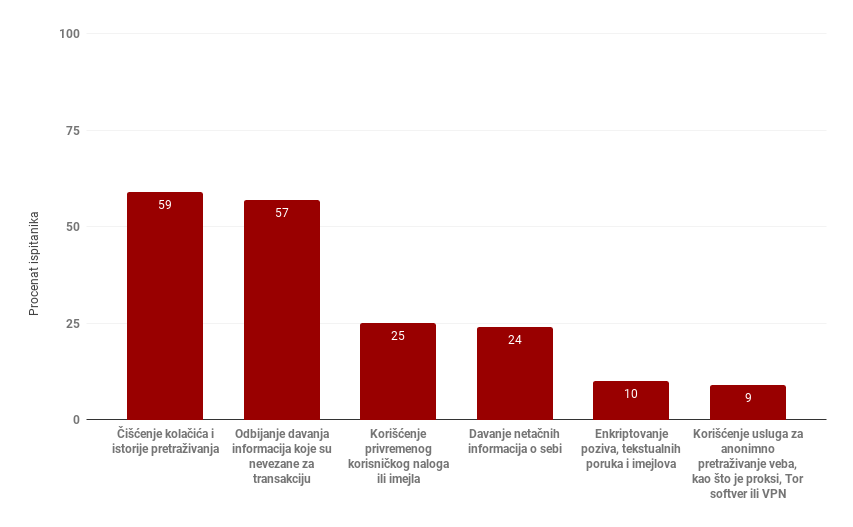
\includegraphics[scale=0.35]{chart.png}
	\end{center}
	\caption{Procenat u kome se preduzimaju određene mere zaštite privatnosti}
	\label{fig:slika1}
\end{figure}

\subsection{Enkripcija} 
Internet je otvoren sistem, što znači da se svi podaci kroz više uređaja, deljenih konekcija, ili čak bežično šalju kako bi stigli do željene destinacije. Ovime se omogućava komunikacija između nekoliko uređaja koji mogu biti udaljeni više hiljada kilometara. Ovaj vid komunikacije sa sobom nosi vidne prednosti, ali zbog načina na koji je organizovan, i vidne probleme. Kako je komunikacija između početnog i krajnjeg uređaja posredovana mnogim uređajima, svaki uređaj u sredini može videti šta je poslato. To znači da je svaka ukucana lozinka ili broj kreditne kartice vidljiv uređajima kojima nije namenjen i od kojih bi trebalo da bude sakriven. U svrhe prevazilaženja ovog problema koristi se enkripcija. Enkripcija je mehanizam kojim se bilo kakva informacija šifruje, tj. prebacuje iz čitljivog oblika u naizgled nasumične karaktere, koji se uz pomoć odgovarajućeg ključa mogu vratiti u svoj prvobitan oblik \cite{dataencryption}. 
\par Enkripcija na internetu prilično je česta i uobičajena pojava. Svakim učitavanjem “https” stranice na internetu veb pregledač uspostavlja enkriptovanu komunikaciju sa serverom na kome se ta stranica nalazi \cite{enc1}. Tekst, slike i video zapisi šifruju se tako da informaciju u prvobitan oblik ne bi mogao vratiti niko ko bi pokušao da je presretne. Tek kada stranica stigne do primaoca kome je namenjena, veb pregledač dešifruje te informacije tako da cela strana ponovo postane čitljiva. Slično tome, pri dopisivanju preko aplikacija za ćaskanje kao sto su Fejsbuk, Vatsap, Vajber i mnoge druge, uspostavlja se takozvana “end-to-end” enkripcija koja omogućava da sadržaj razmenjivanih poruka osim pošaljioca i primaoca ne može videti niko, pa čak ni sami serveri koji tu komunikaciju omogućavaju \cite{enc2}. Uz to, postoje i specijalizovani veb pregledači, kao što je Tor, koji omogućava pretraživanje uz enkripciju upita \cite{enc3}. Tor koristi višeslojnu enkripciju tako što se enkriptovani sadržaj šalje od čvora do čvora i postepeno dekriptuje dok ne stigne do odredišta.
\par Prema tome, neki sajtovi koriste enkripciju kako bi čuvali podatke svojih korisnika, te se privatnost koju garantuju ovi sajtovi zasniva upravo na njoj. S tim u vezi, ukoliko pojedinac želi da bude siguran da su podaci koje ostavlja negde na internetu sigurni, jedan od koraka koji može preduzeti je upravo provera da li sajt koristi neki vid enkripcije, kako bi odlučio da li je bezbedno da svoje podatke ostavi na njemu. 


\subsection{Virtuelne privatne mreže (VPN)}
\label{subsec:vpn}

Virtuelne privatne mreže (eng.~{\em virtual private network, VPN}) nastale su usled potrebe da se biznisi, organizacije, vlade i slični subjekti koji poseduju osetljive informacije zaštite od hakovanja i gubitka podataka u slučajevima kada je potrebno da im udaljeni korisnici ili satelitske kancelarije pristupe, kao i radi smanjenja telekomunikacionih troškova efikasnijim korišćenjem infrastrukture.\textit{ "VPN su privatne mreže koje rade preko deljene javne infrastrukture kao što je Internet"} \cite{vpn2}. Virtuelna je zato što ne postoji odvojena fizička infrastruktura za datu mrežu, već koristi već postojeću javnu infrastrukturu. Privatna je zato što  omogućava bezbednu upotrebu uz garanciju da će samo članovi mreže moći da vide poslate informacije \cite{vpn3}. VPN omogućavaju privatnost podataka korišćenjem sigurnosnih procedura (enkripcija) i protokola tuneliranja (IPsec, PPTP, L2TP). Pod tuneliranjem se podrazumeva da VPN pravi "tunel" između korsinika pri čemu se podaci enkriptuju na strani pošiljaoca, šalju kroz tunel i zatim dekriptuju na strani primaoca. Pored podataka mogu se enkriptovati i polazna i završna adresa radi veće sigurnosti \cite{vpn4}. 
\par Usled skorašnjih otkrića o velikim projektima za nadzor i usled ograni-\\čenja koje određene vlade nameću svojim građanima, sve više raste upotreba VPN usluga. Iako to nije bila njihova prvobitna namena, VPN usluge se sve više koriste za zaštitu privatnosti pojedinaca, kao i za zaštitu od cenzurisanja, a i za pristup sadržaju koji je geografski ograničen. Još jedan od razloga za povećano korišćenje je porast upotrebe javnih mreža koje je prouzrokovano širenjem mobilne industrije, što je dovelo do stvaranja uslova za napade, kao što su krađa akreditiva, presretanje paketa i krađa sesija. Ovo dovodi do toga da neki korisnici koriste VPN za zaštitu svojih interakcija \cite{vpn5}. Danas postoji veliki broj komercijalnih VPN provajdera čije usluge variraju od besplatnih (Windscribe, TunnelBear) do skupih i bezbednijih (ExpressVPN, NordVPN, IPVanish). Na korisniku je samo da izabere provajdera i pre pristupa internetu aktivira VPN i time poveća bezbednost prenesenih podataka, finansijskih transakcija i privatnih informacija i time se zaštiti od mogućih presretanja i/ili zloupotrebe podataka. VPN takođe pruža zaštitu od krađe identiteta i sakriva IP adresu, čime trećim licima otežava praćenje. 
\par Iako VPN provajderi pružaju navedene usluge do nekog stepena, dovodi se u pitanje njihova sposobnost da očuvaju anonimnost i privatnost. Privatnost se kod ovih mreža ne odnosi na privatnost krajnjih korisnika već na povezivanje više privatnih mreža. Zbog lakoće korišćenja, velikih performansi i jakog marketinga postoji velika privlačnost ovih mreža, ali neinformisanost korisnika može dovesti do problema pri korišćenju. Iako veliki broj pružalaca VPN usluga  tvrde da pružaju robusne i sigurne infrastrukture tako što ne loguju podatke korisnika, na osnovu sprovedenog istraživanja gde je evaluirano 62 komercijalna VPN provajdera utvrđeno je da oko 10\% VPN servisa presreću i/ili manipulišu saobraćajem \cite{vpn6}.

 
\section{Zaključak}
\label{sec:zakljucak}
Ovaj rad je imao za cilj da predstavi izazove sa kojima se korisnici interneta suočavaju, a koji se tiču privatnosti njihovih podataka. Kao što je prethodno izneto, ljudi nisu svesni da su njihovi podaci u opasnosti, iako često izveštavaju o tome da su zabrinuti povodom toga ko sve ima pristup njihovim privatnim podacima. S tim u vezi, cilj rada bio je i da skrene pažnju na to kako su, čak i kada nam provajderi usluga tvrde suprotno, naše informacije konstantno pod rizikom iskorišćavanja od strane drugih ljudi ili velikih kompanija. Uz to, rad je imao za cilj i da ukaže na potrebu da se kritički pristupi obećanjima i ugovorima koje pružaju provajderi usluga, s obzirom da nalazi uključuju i da je praksa različita od načelnih obećanja o čuvanju privatnosti. Na kraju, dat je i pregled dve tehnike zaštite privatnosti koje su prisutne na internetu. Kao što su informacije iznete u radu pokazale, polje privatnosti na internetu otvara mnoga pitanja za razmatranje, od kojih je jedno od najvažnijih to da li u ovom trenutku razvoja tehnologije možemo uopšte da govorimo o privatnosti na internetu. S tim u vezi, naš stav je da je privatnost moguće zaštiti, ali da to zahteva veliki napor i informisanost pojedinca. Odnosno, pojedincu privatnost nije zagarantovana, već on mora aktivno da radi na njenom obezbeđivanju. Zbog toga bi u budućnosti trebalo razmotriti načine na koji se ljudi mogu informisati o svojim pravima i obavezama, tako da bi mogli da donose informisane odluke o tome kada i kako da se odreknu svoje privatnosti, ili da je pak zadrže.

\addcontentsline{toc}{section}{Literatura}
\bibliography{seminarski} 
\bibliographystyle{plain}



\end{document}
